\setcounter{dang}{0}
\newpage
\section{CÔNG THỨC TÍNH GÓC TRONG KHÔNG GIAN}
\subsection{LÝ THUYẾT CẦN NHỚ}
\subsubsection{Góc giữa hai mặt phẳng}
\begin{itemize}
	\item [\iconMT] \indam{Công thức:} Gọi $\vec{n_1}=(a_1;b_1;c_1)$, $\vec{n_2}=(a_2;b_2;c_2)$ lần lượt là vectơ pháp tuyến của $(P)$ và $(Q)$; $\varphi$ là góc giữa hai mặt phẳng $(P)$ và $(Q)$, với $0^\circ \leq \varphi \leq 90^\circ$.
	Khi đó
	\boxmini{$\cos \varphi =\bigg|\cos\left(\vec{n_1}, \vec{n_2}\right) \bigg| =\dfrac{\bigg|a_1a_2+b_1b_2+c_1c_2\bigg|}{\sqrt{a_1^2+b_1^2+c_1^2} \cdot \sqrt{a_2^2+b_2^2+c_2^2}}$}
	\item [\iconMT] \indam{Chú ý:}
	\begin{itemize}
		\item [$\bullet$] Nếu $(P)$ song song hoặc trùng $(Q)$ thì $\varphi =0^\circ$.
		\item [$\bullet$] Nếu $(P)\perp (Q)$ thì $\varphi =90^\circ$. Khi đó $\vec{n_1}\cdot \vec{n_2}=0 \Leftrightarrow a_1a_2+b_1b_2+c_1c_2=0$.
	\end{itemize}
\end{itemize}
\subsubsection{Góc giữa hai đường thẳng}
\begin{itemize}
	\item [\iconMT] \indam{Công thức:}  Gọi $\vec{u}=(u_1;u_2;u_3)$, $\vec{v}=(v_1;v_2;v_3)$ lần lượt là vectơ chỉ phương của  $d_1$ và $d_2$; $\varphi$ là góc giữa hai đường thẳng $d_1$ và $d_2$, với $0^\circ \leq \varphi \leq 90^\circ$.
	Khi đó
	\boxmini{$\cos \varphi =\bigg|\cos\left(\vec{u}, \vec{v}\right) \bigg| =\dfrac{\bigg|u_1v_1+u_2v_2+u_3v_3\bigg|}{\sqrt{u_1^2+u_2^2+u_3^2} \cdot \sqrt{v_1^2+v_2^2+v_3^2}}$}
	\item [\iconMT] \indam{Chú ý:}
	\begin{itemize}
		\item [$\bullet$] Nếu $d_1$ song song hoặc trùng $d_2$ thì $\varphi =0^\circ$.
		\item [$\bullet$] Nếu $d_1\perp d_2$ thì $\varphi =90^\circ$. Khi đó $\vec{u} \cdot\vec{u} =0 \Leftrightarrow u_1v_1+u_2v_2+u_3v_3=0$.
	\end{itemize}
\end{itemize}

\subsubsection{Góc giữa đường thẳng và mặt phẳng}
\begin{itemize}
	\item [\iconMT] \indam{Công thức:}  Gọi $\vec{u}=(u_1;u_2;u_3)$, $\vec{n}=(A;B;C)$ lần lượt là vectơ chỉ phương của  $d$ và vectơ pháp tuyến của $(P)$; $\varphi$ là góc giữa đường thẳng $d$ và mặt phẳng $(P)$, với $0^\circ \leq \varphi \leq 90^\circ$.
	Khi đó
	\boxmini{$\sin \varphi =\bigg|\cos\left(\vec{u}, \vec{n}\right) \bigg| =\dfrac{\bigg|u_1A+u_2B+u_3C\bigg|}{\sqrt{u_1^2+u_2^2+u_3^2} \cdot \sqrt{A^2+B^2+C^2}}$}
	\item [\iconMT] \indam{Chú ý:}
	\begin{itemize}
		\item [$\bullet$] Nếu $d$ song song hoặc trùng $(P)$ thì $\varphi =0^\circ$, khi đó $\vec{u} \perp \vec{n}$
		\item [$\bullet$] Nếu $d$ vuông góc với $(P)$ thì $\varphi =90^\circ$, khi đó $\vec{u} =k \cdot \vec{n}$.
	\end{itemize}
\end{itemize}
\subsection{PHÂN LOẠI, PHƯƠNG PHÁP GIẢI TOÁN}
\begin{dang}{Tính góc trong không gian Oxyz}
	\begin{itemize}
		\item [$\bullet$] Xác định vectơ chỉ phương (vectơ pháp tuyến);
		\item [$\bullet$] Áp dụng đúng công thức.
	\end{itemize}
\end{dang}
\boxmini{BÀI TẬP TỰ LUẬN}
\setcounter{vd}{0}
\begin{vd}
	Trong không gian $Oxyz$, tính góc giữa hai mặt phẳng sau:
	\begin{enumEX}[a)]{1}
		\item $(P)\colon x+y+4z-2=0$ và $(Q)\colon 2x-2z+7=0$.
		\item $(P)\colon 2x - y-2z-9=0$ và $(Q)\colon  x - y - 6=0$.
	\end{enumEX}
	\loigiai
	{
	\begin{enumEX}[a)]{1}
		\item Ta có $\vec{n}_P=(1;1;4)$, $\vec{n}_Q=(2;0;-2)$ lần lượt là vectơ pháp tuyến của $(P)$ và $(Q)$.\\
		Suy ra $\cos\left((P),(Q)\right)=|\cos\left(\vec{n}_P,\vec{n}_Q\right)|=\dfrac{|\vec{n}_P\cdot \vec{n}_Q|}{|\vec{n}_P|\cdot |\vec{n}_Q|}=\dfrac{|2+0-8|}{\sqrt{18}\cdot \sqrt{8}}=\dfrac{1}{2}$.\\
		Vậy góc giữa $(P)$ và $(Q)$ bằng $60^\circ$.
		\item $(P)\colon 2x - y-2z-9=0$ có $1$ vectơ pháp tuyến là $\overrightarrow{n_1} = (2;-1;-2)$.\\
		$(Q)\colon  x - y - 6=0$ có $1$ vectơ pháp tuyến là $\overrightarrow{n_2} = (1;-1;0)$.\\
		$\cos \left(\left( P \right);\left( Q \right)\right) = \dfrac{\left|\overrightarrow{n_1}, \overrightarrow{n_2}\right|}{\left|\overrightarrow{n_1}\right|\left|\overrightarrow{n_2}\right|} $
		$= \dfrac{\left|2\cdot 1 + \left(- 1\right)\left(- 1\right) + 0\right|}{\sqrt{2^2 + 1^2 + 2^2}\cdot \sqrt{1^2+ 1^2 + 0}}= \dfrac{1}{\sqrt{2}} \Rightarrow \left(\left( P \right);\left( Q \right)\right) = 45^\circ$.
	\end{enumEX}
	}
\end{vd}
\dongcham{10}
\begin{vd}%[Phan Quốc Trí]%[2H3B3-4]%
	Trong không gian $Oxyz$, tính góc giữa hai đường thẳng sau:
	\begin{enumEX}[a)]{1}
		\item $d:\heva{&x=1-t\\&y=t \\&z=0}$ và $d': \dfrac{x}{-2}=\dfrac{y}{1}=\dfrac{z-1}{-2}$.
		\item $d_1\colon \heva{&x=2+t\\&y=-1+t\\&z=3}$ và $ d_2\colon \heva{&x=1-t'\\&y=2\\&z=-2+t'}$. 
	\end{enumEX} 
	\loigiai{
		\begin{enumEX}[a)]{1}
			\item Gọi $\varphi$ là góc giữa hai đường thẳng $d$ và $d'$. Ta có
			$$\cos \varphi = \dfrac{\left| (-1)\cdot (-2) + 1 \cdot 1+0\cdot (-2) \right|}{\sqrt{(-1)^2+1^2+0^2}\cdot \sqrt{(-2)^2+1^2+(-2)^2}} = \dfrac{\sqrt{2}}{2} \Rightarrow \varphi = 45^{\circ}.$$
			\item $d_1$ có VTCP $\overrightarrow{v}_1=(1;1;0)$ và $d_2$ có VTCP $\overrightarrow{v}_2=(-1;0;1)$, $\left|v_1 \right|=\sqrt{2} $, $\left|v_2 \right|=\sqrt{2}$.\\
			Khi đó góc giữa hai đường thẳng $d_1$ và $d_2$ là
			\[\cos \left(d_1, d_2 \right)=\dfrac{\left|\overrightarrow{v}_1\cdot \overrightarrow{v}_2 \right|}{\left|\overrightarrow{v}_1 \right|\cdot\left|\overrightarrow{v}_2 \right|}=\dfrac{1}{2}. \]
			Vậy góc giữa hai đường thẳng $d_1$ và $d_2$ là $60^\circ$.
		\end{enumEX}
	}
\end{vd}
\dongcham{10}
\begin{vd}%[2H3B3-4]%
	Trong không gian $Oxyz$, tính góc giữa đường thẳng và mặt phẳng sau:
	\begin{enumEX}[a)]{1}
		\item $d\colon\dfrac{x-1}{1}=\dfrac{y}{2}=\dfrac{z+1}{-1}$ và $(P)\colon x-y+2z+1=0$.
		\item $d\colon \dfrac{x-1}{4}=\dfrac{y-6}{3}=\dfrac{z+4}{1}$ và $(P)\colon 4x+3y-z+1=0$
	\end{enumEX}
	\loigiai{
		\begin{enumEX}[a)]{1}
			\item Ta có $\overrightarrow{n}_{(P)}=(1;-1; 2)$ và $\overrightarrow{u}_d=(1; 2;-1)$.\\
			Vậy $\sin\left(d;(P)\right)=\dfrac{\left|\overrightarrow{n}_{(P)}\cdot\overrightarrow{u}_d\right|}{\left|\overrightarrow{n}_{(P)}\right|\cdot\left|\overrightarrow{u}_d\right|} =\dfrac{|1-2-2|}{\sqrt{6}\cdot\sqrt{6}}=\dfrac{1}{2}\Rightarrow \left(d;(P)\right)=30^{\circ}$.
			\item Mặt phẳng $(P)$ có vectơ pháp tuyến $\overrightarrow{n}=(4;3;-1)$.\\
			Đường thẳng $d$ có vectơ chỉ phương $\overrightarrow{u}=(4;3;1)$.\\
			Gọi $\alpha$ là góc giữa $d$ và $(P)$, ta có $\sin\alpha=\dfrac{\left|\overrightarrow{n}\cdot \overrightarrow{u}\right|}{\left|\overrightarrow{n}\right|\cdot \left|\overrightarrow{u}\right|}=\dfrac{|16+9-1|}{\sqrt{16+9+1}\cdot \sqrt{16+9+1}}=\dfrac{12}{13} \Rightarrow \alpha \approx 67,38^\circ$.
		\end{enumEX}
		}
\end{vd}
\dongcham{17}
\boxmini{BÀI TẬP TRẮC NGHIỆM}
\setcounter{ex}{0}
\Opensolutionfile{ans}[ans/2H5-B3-d1]
\begin{ex}
	Cho mặt phẳng $(P):x+2y-2z+3=0$, mặt phẳng $(Q):x-3y+5z-2=0$. Cosin của góc giữa hai mặt phẳng $(P)$, $(Q)$ là
	\choice
	{$-\dfrac{\sqrt{35}}{7}$}
	{$\dfrac{5}{7}$}
	{\True $\dfrac{\sqrt{35}}{7}$}
	{$-\dfrac{5}{7}$}
	\loigiai{
		Mặt phẳng $(P)$ có ve-tơ pháp tuyến là $\overrightarrow{n}_1=(1;2;-2)$\\
		Mặt phẳng $(Q)$ có vec-tơ pháp tuyến là $\overrightarrow{n}_2=(1;-3;5)$.\\
		Ta có $\cos[(P),(Q)]=\left|\cos(\overrightarrow{n}_1,\overrightarrow{n}_2)\right|=\dfrac{|\overrightarrow{n}_1\cdot\overrightarrow{n}_2|}{|\overrightarrow{n}_1|\cdot|\overrightarrow{n}_2|}=\left|\dfrac{-15}{3\sqrt{35}}\right|=\dfrac{\sqrt{35}}{7}$.}
\end{ex}

\begin{ex}
	Góc giữa hai mặt phẳng $(P):x+2y+z+4=0$ và $(Q):-x+y+2z+3=0$ bằng
	\choice
	{$45^{\circ}$}
	{$90^{\circ}$}
	{$30^{\circ}$}
	{\True $60^{\circ}$}
	\loigiai{
		Gọi $\varphi$ là góc giữa $(P)$ và $(Q)$. Ta có
		$$\cos \varphi = \dfrac{\left| 1\cdot (-1)+2\cdot 1+1\cdot 2 \right|}{\sqrt{1^2+2^2+1^2} \cdot \sqrt{(-1)^2 +1^2+2^2}}=\dfrac{1}{2} \Rightarrow \varphi = 60^{\circ}.$$
	}
\end{ex}

\begin{ex}
	Tính góc $\alpha$ giữa mặt $(P)\colon x+z-4=0$ và mặt phẳng $(Oxy)$.
	\choice
	{\True $45^\circ$}
	{$30^\circ$}
	{$90^\circ$}
	{$60^\circ$}
	\loigiai{
		Ta có $\vec{n}_{(P)}=(1;0;1)$, $\vec{n}_{(Oxy)}=(0;0;1)$.\\
		Suy ra $\cos \alpha =\dfrac{\left| 1\cdot 0+0\cdot 0+1\cdot 1 \right|}{\sqrt{2}\cdot \sqrt{1}}=\dfrac{\sqrt{2}}{2}$.\\
		Vậy $\widehat{((P);(Q))}=45^\circ$.
	}
\end{ex}

\begin{ex}
	Cho điểm $H\left(2;1;2 \right)$, điểm $H$ là hình chiếu vuông góc của gốc tọa độ $O$ xuống mặt phẳng $\left(P \right)$, số đo góc giữa mặt phẳng $\left(P \right)$ và mặt phẳng $\left(Q \right):x+y-11=0$ là
	\choice
	{\True $45^\circ$}
	{$30^\circ$}
	{$60^\circ$}
	{$90^\circ$}
	\loigiai
	{
		Vì điểm $H$ là hình chiếu vuông góc của gốc tọa độ $O$ xuống mặt phẳng $(P)$ nên ta chọn
		$\vec{OH}=\vec{n}_{(P)}=(2;1;2)$.\\
		Phương trình mặt phẳng $(P)$ có dạng
		$$2\left(x-2\right)+\left(y-1\right)+2\left(z-2\right)=0\Leftrightarrow 2x+y+2z-9=0.$$
		Do đó, góc giữa 2 mặt phẳng $(P),(Q)$ tính như sau
		$$\cos \left((P),(Q)\right)=\dfrac{\left|{\vec{n}_{(P)}\cdot\vec{n}_{(Q)}}\right|}{\left|{\vec{n}_{(P)}}\right|\left|{\vec{n}_Q}\right|}=\dfrac{|2\cdot1+1\cdot1+2\cdot0|}{\sqrt{9}\cdot\sqrt{2}}=\dfrac{3}{3\sqrt{2}}=\dfrac{\sqrt{2}}{2}.$$
		Do đó góc giữa mặt phẳng $(P)$ và mặt phẳng $(Q)$ bằng $\cos 45^\circ=\dfrac{\sqrt{2}}{2}$.
	}
\end{ex}


\begin{ex}
	Cho hai đường thẳng $d_1\colon \dfrac{x}{-1}=\dfrac{y+1}{2}=\dfrac{z}{2}$, $d_2\colon\heva{& x=2t \\ & y=1\\ & z=1-t}$. Gọi $\varphi$ là góc
	giữa hai đường thẳng $d_1$, $d_2$. Tính $\cos\varphi$.
	\choice
	{$\cos \varphi=-\dfrac{4\sqrt{5}}{15}$}
	{\True $\cos \varphi=\dfrac{4\sqrt{5}}{15}$}
	{$\cos \varphi=\dfrac{\sqrt{6}}{9}$}
	{$\cos \varphi=-\dfrac{\sqrt{6}}{9}$}
	\loigiai
	{Đường thẳng $d_1$, $d_2$ lần lượt có vectơ chỉ phương là $\overrightarrow{u}_1=(-1; 2; 2)$ và $\overrightarrow{u}_2=(2; 0; -1)$.\\
		Vậy $\cos\varphi=\left|\cos\left(\overrightarrow{u}_1, \overrightarrow{u}_2\right)\right|=\dfrac{|(-1)\times 2 +2\times 0+ 2\times(-1)|}{\sqrt{(-1)^2+2^2+2^2}\cdot\sqrt{2^2+0^2+(-1)^2}}=\dfrac{|-4|}{3\sqrt{5}}=\dfrac{4\sqrt{5}}{15}$.
	}
\end{ex}

\begin{ex}%[2H3B3-4]%
	Cho đường thẳng $d_1\colon \dfrac{x}{-1}=\dfrac{y+1}{1}=\dfrac{z-1}{-2}$ và $d_2\colon \dfrac{x+1}{-1}=\dfrac{y}{1}=\dfrac{z-3}{1}$. Góc giữa hai đường thẳng bằng
	\choice
	{\True $90^\circ$}
	{$30^\circ$}
	{$60^\circ$}
	{$45^\circ$}
	\loigiai{
		Đường thẳng $d_1$ có VTCP là $\vec{a}=(-1;1;-2)$, đường thẳng $d_2$ có VTCP là $\vec{b}=(-1;1;1)$.\\
		Ta có $\vec{a}\cdot \vec{b}= 0\Rightarrow d_1\perp d_2\Rightarrow \left( d_1, d_2\right) =90^\circ$.
	}
\end{ex}

\begin{ex}
	Cho đường thẳng $d$ là giao tuyến của hai mặt phẳng\\ $(P) \colon x-z \cdot \sin \alpha +\cos \alpha =0$ và $(Q) \colon y-z \cdot \cos \alpha -\sin \alpha =0$, $\alpha \in \left(0;\dfrac{\pi}{2}\right)$. Góc giữa $d$ và trục $Oz$ là
	\choice
	{$90^{\circ}$}
	{$30^{\circ}$}
	{\True $45^{\circ}$}
	{$60^{\circ}$}
	\loigiai{
		Xét hệ phương trình $\left\{\begin{aligned}
			&x-z \cdot \sin \alpha +\cos \alpha =0\\
			&y-z \cdot \cos \alpha -\sin \alpha =0\\
		\end{aligned}\right. $. \\
		Ta có $\vec{n}_P=\left(1;0;-\sin \alpha \right)$ và $\vec{n}_Q=\left(0;1;-\cos \alpha \right)$.\\
		vectơ chỉ phương của $d$ là $\vec{u}_d=\left[\vec{n}_P;\vec{n}_Q \right]=\left(\sin \alpha;\cos \alpha;1\right)$.\\
		vectơ chỉ phương của trục $Oz$ là $\vec{k}=(0;0;1)$.\\
		Gọi $\varphi $ là góc giữa đường thẳng $d$ và trục $Oz$.\\
		Ta có $\cos \varphi =\dfrac{\left|\vec{u}_d \cdot \vec{k}\right|}{\left|\vec{u}_d\right| \cdot \left|\vec{k}\right|}=\dfrac{1}{\sqrt{2}}$. Suy ra $\varphi =45^{\circ}$.}
\end{ex}

\begin{ex}%[2-TT-5- Đề thi tháng 2-2019, Toán 12 trường THPT chuyên Bắc Giang- 2019]%[Nguyễn Thế Anh-EX6]%[2H3B3-4]%
	Cho đường thẳng $d\colon \heva{& x=1-t \\ & y=2+2t \\ & z=3+t}$ và mặt phẳng $(P)\colon x-y+3=0$. Tính số đo góc giữa đường thẳng $d$ và mặt phẳng $(P)$.
	\choice
	{$45^\circ$}
	{$120^\circ$}
	{\True $60^\circ$}
	{$30^\circ$}
	\loigiai
	{
		Ta có $\vec {u}=(-1;2;1)$ là vectơ chỉ phương của đường thẳng $d$ và $\vec{n}=(1;-1;0)$ là vectơ pháp tuyến của mặt phẳng $(P)$.\\
		Suy ra $\sin \left(d;(P)\right)=\left|\cos \left(\vec{u};\vec{n}\right)\right|=\dfrac{\left|\vec{u} \cdot \vec{n}\right|}{|\vec{u}|\cdot |\vec{n}|}=\dfrac{\sqrt{3}}{2}$. Vậy $(d;(P))=60^\circ$.
	}
\end{ex}

\begin{ex}
	Cho mặt phẳng $(P)\colon 3x+4y+5z-8=0$ và đường thẳng $d\colon\heva{&x=2-3t\\&y=-1-4t\\&z=5-5t}$. Góc giữa đường thẳng $d$ và mặt phẳng $(P)$ là
	\choice
	{\True $90^{\circ}$}
	{$45^{\circ}$}
	{$30^{\circ}$}
	{$60^{\circ}$}
	\loigiai{
		Mặt phẳng $(P)$ có một vectơ pháp tuyến là $\overrightarrow{n}=(3;4;5)$.\\
		Đường thẳng $d$ có một vectơ chỉ phương là $\overrightarrow{u}=(-3;-4;-5)$.\\
		Ta có $\overrightarrow{n}=-\overrightarrow{u}\Rightarrow d\perp(P)$ nên góc giữa đường thẳng $d$ và mặt phẳng $(P)$ là $90^{\circ}$.
	}
\end{ex}

\begin{ex}
	Cho mặt phẳng $(P)\colon x+y-\sqrt{2}z+5=0$. Tính góc $\varphi$ giữa mặt phẳng $(P)$ và trục $Oy$.
	\choice
	{$\varphi=60^{\circ}$}
	{$\varphi=45^{\circ}$}
	{$\varphi=90^{\circ}$}
	{\True $\varphi=30^{\circ}$}
	\loigiai{
		Ta có vectơ pháp tuyến của mặt phẳng $(P)$ là $\overrightarrow{n}=(1;1;-\sqrt{2})$ và vectơ chỉ phương của trục $Oy$ là $\overrightarrow{u}=(0;1;0)$. Suy ra $\sin\varphi=\dfrac{|\overrightarrow{u}\cdot \overrightarrow{n}|}{|\overrightarrow{u}|\cdot|\overrightarrow{n}|}=\dfrac{|1|}{\sqrt{4}\cdot 1}=\dfrac{1}{2}\Rightarrow\varphi=30^{\circ}$.
	}
\end{ex}


\begin{ex}
	Cho hai mặt phẳng $(P)\colon (m-1)x+y-2z+m=0$ và $(Q)\colon 2x-z+3=0.$ Tìm $m$ để $(P)$ vuông góc với $(Q).$
	\choice
	{\True $m=0$}
	{$m=\dfrac32$}
	{$m=5$}
	{$m=-1$}
	\loigiai{
		$(P)$ vuông góc với $(Q)$ khi và chỉ khi các vectơ pháp tuyến của chúng vuông góc với nhau, tức là $$(m-1;1;-2)\cdot(2;0;-1)=0\Leftrightarrow m=0.$$
	}
\end{ex}

\begin{ex}
	Cho mặt phẳng $(P) \colon x-3y+2z+1=0$ và $(Q) \colon (2m-1)x+m(1-2m)y+(2m-4)z+14=0$ với $m$ là tham số thực. Tổng các giá trị của $m$ để $(P)$ và $(Q)$ vuông góc nhau bằng
	\choice
	{$-\dfrac{3}{2}$}
	{\True $-\dfrac{1}{2}$}
	{$-\dfrac{5}{2}$}
	{$-\dfrac{7}{2}$}
	\loigiai{
		$(P)$ có vectơ pháp tuyến $\overrightarrow{n}_P =(1;-3;2)$.
		\\ $(Q)$ có vectơ pháp tuyến $\overrightarrow{n}_{Q} =\left( 2m-1;m(1-2m);2m-4 \right)$. \\
		$(P)$ và $(Q)$ vuông góc với nhau khi và chỉ khi $\overrightarrow{n}_P \perp \overrightarrow{n}_{Q}$.
		\\ Điều này tương đương với $\overrightarrow{n}_P \cdot \overrightarrow{n}_Q =0 \Leftrightarrow 6m^2+3m -9=0 \Leftrightarrow \hoac{&m=1 \\ &m=-\dfrac{3}{2}.}$
		\\ Tổng các giá trị của $m$ để $(P)$ và $(Q)$ vuông góc nhau bằng $1 -\dfrac{3}{2} = -\dfrac{1}{2}$.
	}
\end{ex}

\begin{ex}%[Trần Bình Thuận - DA2]%[2H3K2-5]% Câu 7
	Cho hai mặt phẳng $ (P)\colon x+2y-z+2=0 $ và $ (Q) \colon x-my+(m+1)z+m-2=0 $, với $ m $ là tham số. Gọi $ S $ là tập hơn tất cả các giá trị của $ m $ sao cho góc giữa $ (P) $ và $ (Q) $ bằng $ 60^{\circ} $. Tính tổng các phần tử của $ S $.
	\choice
	{$ 1 $}
	{$ -\dfrac{1 }{2} $}
	{$ \dfrac{3 }{2} $}
	{\True $ \dfrac{1 }{2} $}
	\loigiai{
		vectơ pháp tuyến của mặt phẳng $ (P): \vec{n}_{(P)} = (1;2;-1) $.\\
		vectơ pháp tuyến của mặt phẳng $ (Q): \vec{n}_{(Q)} = (1;-m;m+1) $.\\
		Góc giữa hai mặt phẳng $ (P) $ và $ (Q) $ bằng $ 60^{\circ} $ nên
		{\allowdisplaybreaks
			\begin{eqnarray*}
				&&\dfrac{|1-2m-m-1|}{\sqrt{6}\cdot\sqrt{2m^2+2m+2}}= \cos 60^{\circ}\\
				&\Leftrightarrow& |3m| = \dfrac{1}{2}\sqrt{6}\cdot\sqrt{2m^2+2m+2}\\
				&\Leftrightarrow& 9m^2 = 3(m^2+m+1)\\
				&\Leftrightarrow& 2m^2-m-1=0 \Leftrightarrow \hoac{&m=1\\&m=-\dfrac{1}{2}.}
		\end{eqnarray*}}
		Do đó $ S=1+\left( -\dfrac{1}{2} \right) =\dfrac{1}{2} $.
	}
\end{ex}

\begin{ex}
	Hãy tìm tham số thực $m$ để góc giữa hai đường thẳng  sau bằng $60^\circ$.
	$$d\colon \heva{&x=1+t\\&y=-\sqrt{2}t\\&z=1+t}\, ,t\in \mathbb{R} \text {và } d'\colon \heva{&x=1+t'\\&y=1+\sqrt{2}t'\\&z=1+mt'}\, , t'\in \mathbb{R}$$ 
	\choice
	{$\dfrac{1}{2}$}
	{$-1$}
	{\True $-\dfrac{1}{2}$}
	{$1$}
	\loigiai{
		Ta có $\heva{&\vec{u}_d=(1;-\sqrt{2};1)\\&\vec{u}_{d'}=(1;\sqrt{2};m)}\Rightarrow	\cos\alpha = \dfrac{\left|-1+m\right| }{\sqrt{4}\cdot \sqrt{3+m^2}}$
		\begin{eqnarray*}
			\cos\alpha = \cos 60^\circ &\Leftrightarrow& \dfrac{\left|-1+m\right| }{\sqrt{4}\cdot \sqrt{3+m^2}}=\dfrac{1}{2}\\
			&\Leftrightarrow& |-1+m|=\sqrt{3+m^2}\\
			&\Leftrightarrow& -2m+2=0\\
			&\Leftrightarrow& m=1
		\end{eqnarray*}
	}
\end{ex}

\begin{ex}
	Cho các điểm $A(-1;\sqrt{3};0)$, $B(1;\sqrt{3};0)$, $C(0;0;\sqrt{3})$ và điểm $M$ thuộc trục $Oz$ sao cho hai mặt phẳng $(MAB)$ và $(ABC)$ vuông góc với nhau. Tính góc giữa hai mặt phẳng $(MAB)$ và $(OAB)$.
	\choice
	{\True $45^\circ$}
	{$60^\circ$}
	{$15^\circ$}
	{$30^\circ$}
	\loigiai{
		$M(0;0;m)$ thuộc trục $Oz$.\\
		Ta có $\vv{AM}=(1;-\sqrt{3};m)$, $\vv{AB}=(2;0;0)$, $\vv{AC}=(1;-\sqrt{3};\sqrt{3})$.\\
		$\Rightarrow \vv{n}_1 =\left[ \vv{AB}, \vv{AC} \right] =(0;-2\sqrt{3};-2\sqrt{3})$,
		$\vv{n}_2 =\left[ \vv{AB}, \vv{AM} \right] =(0;-2m;-2\sqrt{3})$.\\
		Mặt phẳng $(ABC)$ có một vectơ pháp tuyến là $\vv{n}_1$, mặt phẳng $(MAB)$ có một vectơ pháp tuyến là $\vv{n}_2$.\\
		Hai mặt phẳng $(MAB)$ và $(ABC)$ vuông góc với nhau khi và chỉ khi
		$$\vv{n}_1 \perp \vv{n}_2
		\Leftrightarrow 0\cdot 0  +(-2\sqrt{3})\cdot (-2m) + (-2\sqrt{3})\cdot (-2\sqrt{3}) =0
		\Leftrightarrow m=-\sqrt{3}.$$
		Mặt phẳng $(OAB)$ có một vectơ pháp tuyến là $\vv{n}_3 = \left[ \vv{OA}, \vv{OB} \right] =(0;0;-2\sqrt{3})$.\\
		Gọi $\varphi$ là góc giữa hai mặt phẳng $(MAB)$ và $(OAB)$. Khi đó
		$$\cos \varphi =\left| \cos \left( \vv{n}_2, \vv{n}_3 \right) \right|
		= \dfrac{\left| \vv{n}_2 \cdot \vv{n}_3 \right|}{\left| \vv{n}_2 \right| \cdot \left| \vv{n}_3 \right|}
		=\dfrac{12}{2\sqrt{6} \cdot 2\sqrt{3}} =\dfrac{1}{\sqrt{2}}.$$
		Vậy góc giữa hai mặt phẳng $(MAB)$ và $(OAB)$ là $45^\circ$.
	}
\end{ex}



\Closesolutionfile{ans}
\begin{dang}{Tọa độ hóa một số bài toán hình không gian}
\end{dang}

\boxmini{BÀI TẬP TỰ LUẬN}
\setcounter{vd}{0}

\begin{vd}%[2H5V1-6]
	Cho hình lăng trụ đứng $OBC.O'B'C'$ có đáy là tam giác $OBC$ vuông tại $O$ và có $OB=3a$, $OC=a$, $OO'=2a$. Tính góc giữa
	\begin{enumerate}
		\item hai đường thẳng $BO'$ và $B'C$;
		\item hai mặt phẳng $(O'BC)$ và $(OBC)$;
		\item đường thẳng $B'C$ và mặt phẳng $(O'BC)$.
	\end{enumerate}
	\loigiai
	{
		\immini{
			Xét hệ trục tọa độ $Oxyz$ sao cho các điểm có tọa độ như sau: $O(0;0;0)$, $O'(2a;0;0)$, $B(0;3a;0)$, $C(0;0;1a)$.\\
			Trong không gian $Oxyz$ vừa chọn, ta có $B'(2a;3a;0)$, $C'(2a;0;1a)$, $\overrightarrow{BO}'=(0;-3a;0)$, $\overrightarrow{CB}'=(2a;3a;-a)$.
			\begin{enumerate}
				\item Hai đường thẳng $BO'$ và $B'C$ có vectơ chỉ phương lần lượt là $\overrightarrow{u}=(0;3;0)$, $\overrightarrow{v}=(2;3;-1)$.\\
				Ta có 
				\begin{eqnarray*}
					\cos (BO',B'C)&=&\dfrac{\left |\overrightarrow{u}\cdot\overrightarrow{v} \right |}{\left |\overrightarrow{u} \right |\cdot\left |\overrightarrow{v} \right |}\\&=&\dfrac{\left |0\cdot 2+3\cdot 3+0\cdot (-1) \right |}{\sqrt{3^2}\cdot\sqrt{2^2+3^2+(-1)^2}}=\dfrac{3}{\sqrt{14}}.
				\end{eqnarray*}
				Suy ra $(BO',B'C)\approx 36^{\circ}42'$.
				\item Ta có phương trình mặt phẳng $(O'BC)$ theo đoạn chắn là $\dfrac{x}{2a}+\dfrac{y}{3a}+\dfrac{z}{a}=1$ hay $3x+2y+6z-6a=0$.
			\end{enumerate}
		}{
			\begin{tikzpicture}[line cap=round,line join=round,scale=.8,>=stealth,font=\footnotesize ]
				\coordinate (O) at (0,0);
				\coordinate (O') at (0,4.5);
				\coordinate (B) at (5.5,0);
				\coordinate (C) at (2,-2);
				\coordinate (C') at ($(C)+(0,4.5)$);
				\coordinate (B') at ($(B)+(0,4.5)$);
				\coordinate (y) at ($(O)!1.3!(B)$);
				\coordinate (x) at ($(O)!1.3!(O')$);%trung điểm
				\coordinate (z) at ($(O)!1.5!(C)$);%trung điểm
				\draw (B')--(C)--(O')--(B')--(C')--(C)--(B)--(B')(B)--(C')--(O')--(O)--(C)(O)--(C');
				\draw[dashed](O)--(B)--(O');
				\foreach \x/\g in {O'/180,B'/75,C'/180,O/180,B/-80,C/-100}
				\fill[black](\x) circle (1pt)
				($(\x)+(\g:3mm)$) node{\x};
				\draw[->](B)--(y)node[below]{$y$};
				\draw[->](O')--(x)node[above]{$x$};
				\draw[->](C)--(z)node[below right]{$z$};
			\end{tikzpicture}
		}
		Mặt phẳng $(O'BC)$ có vectơ pháp tuyến $\overrightarrow{n}=(3;2;6)$, mặt đáy $(OBC)$ có vectơ pháp tuyến $\overrightarrow{k}=(0;0;1)$. Gọi $\alpha$ là góc giữa mặt phẳng $(O'BC)$ và mặt đáy.\\
		Ta có $\cos\alpha =\dfrac{\left |\overrightarrow{n}\cdot\overrightarrow{k} \right |}{\left |\overrightarrow{n} \right |\cdot\left |\overrightarrow{k} \right |}=\dfrac{\left |3\cdot 0+2\cdot 0+6\cdot 1 \right |}{\sqrt{3^2+2^2+6^2}\cdot\sqrt{1^2}}=\dfrac{6}{7}$.\\
		Suy ra $\left ((O'BC),(OBC) \right )\approx 31^{\circ}1'$.
		\begin{enumerate}
			\setcounter{enumi}{2}
			\item Gọi $\beta$ là góc giữa đường thẳng $B'C$ và mặt phẳng $(O'BC)$.\\
			Ta có $\sin\beta =\dfrac{\left |\overrightarrow{v}\cdot\overrightarrow{n} \right |}{\left |\overrightarrow{v} \right |\cdot\left |\overrightarrow{n} \right |}=\dfrac{\left |2\cdot 3+3\cdot 2+(-1)\cdot 6 \right |}{\sqrt{2^2+3^2+(-1)^2}\cdot\sqrt{3^2+2^2+6^2}}=\dfrac{3\sqrt{14}}{49}$.\\
			Suy ra $(B'C,(O'BC))\approx 13^{\circ}15'$.
		\end{enumerate}
	}
\end{vd}
\dongcham{31}
\begin{vd}%[2H5H2-7]
	Cho hình chóp $S.ABCD$ có đáy $ABCD$ là hình vuông cạnh bằng $4$. Mặt bên $SAB$ là tam giác cân tại $S$ có chiều cao bằng $6$ và nằm trong mặt phẳng vuông góc với đáy.
	\begin{listEX}  
		\item Tính góc $\alpha$ giữa hai đường thẳng $SD$ và $BC$;
		\item Tính góc $\beta$ giữa hai mặt phẳng $(SAD)$ và $(SCD)$.
	\end{listEX}
	\loigiai{
		\immini{Gọi $O$ là trung điểm của $AB$ suy ra $SO\perp(ABCD)$.\\
			Chọn hệ trục $Oxyz$ như hình bên. Ta có: $S(0;0;6)$, $A(2; 0; 0)$, $B(-2; 0; 0)$, $C(-2; 4; 0)$, $D(2; 4; 0)$.}
		{\begin{tikzpicture}[scale=.7,>=stealth, font=\footnotesize, line join=round, line cap=round]
				\coordinate (O) at (0, 0);
				\coordinate (I) at (4, 0);
				\coordinate (S) at (0,6);
				\coordinate (A) at (-1, -1);
				\coordinate (B) at (1, 1);
				\coordinate (C) at (5, 1);
				\coordinate (D) at ($(A)+(C)-(B)$);
				%\draw[color=gray!50,dashed] (\xmin,\ymin) grid (\xmax,\ymax);
				\draw[dashed](A)node[below]{$A$}--(B)node[above right]{$B$}--(C)node[right]{$C$}(O)--(S)node[right]{$S$}--(B)(O)node[left]{$O$}--(I)node[below ]{$I$};
				\draw(S)node[left]{$6$}--(A)node[above left]{$2$}--(D)--(C)--(S)--(D)node[below]{$D$};
				\draw[->](S)--++(0,1)node[left]{$z$};
				\draw[->](I)node[above]{$4$}--++(1,0)node[above]{$y$};
				\draw[->](A)--++(-1,-1)node[left]{$x$};
		\end{tikzpicture}}
		\begin{listEX}
			\item Ta có $\overrightarrow{SD}=(2;4;-6)$, $\overrightarrow{BC}=(0; 4; 0)$, suy ra
			\begin{eqnarray*}
				&\cos \alpha & =\dfrac{|\overrightarrow{S D} \cdot \overrightarrow{B C}|}{|\overrightarrow{S D}| \cdot|\overrightarrow{B C}|}=\dfrac{|2 \cdot 0+4 \cdot 4-6 \cdot 0|}{\sqrt{2^2+4^2+(-6)^2} \cdot \sqrt{4^2}} \\
				&& =\dfrac{\sqrt{14}}{7} \Rightarrow \alpha=57{,}7^{\circ}.
			\end{eqnarray*}
			\item Mặt phẳng $(S A D)$ có cặp vectơ chỉ phương là $\overrightarrow{S D}=(2; 4;-6)$,\\        
			$\overrightarrow{S A}=(2; 0;-6)$ nên có vectơ pháp tuyến $\overrightarrow{n}=-\dfrac{1}{8}[\overrightarrow{S D}, \overrightarrow{SA}]=(3; 0; 1)$.\\     
			Mặt phẳng $(SCD)$ có cặp vectơ chỉ phương là $\overrightarrow{SD}=(2; 4;-6)$,   $\overrightarrow{D C}=(-4; 0; 0)$ nên có vectơ pháp tuyến $\overrightarrow{u}=\dfrac{1}{8}[\overrightarrow{S D}, \overrightarrow{D C}]=(0; 3; 2)$.\\
			Suy ra $\cos \beta=\dfrac{\left|\overrightarrow{n} \cdot \overrightarrow{u}\right|}{|\overrightarrow{n}| \cdot\left|\overrightarrow{u}\right|}=\dfrac{|3 \cdot 0+0\cdot 3+1 \cdot 2|}{\sqrt{3^2+1^2} \cdot \sqrt{3^2+2^2}}=\dfrac{2}{\sqrt{130}} \Rightarrow \beta \approx 79{,}9^{\circ}$.
		\end{listEX}
	}
\end{vd}
\dongcham{15}

\begin{vd}%[2H5V2-8]
	\immini{Người ta muốn dựng một cột ăng-ten trên một sườn đồi. Ăng-ten được dựng thẳng đứng trong không gian $Oxyz$ với độ dài đơn vị trên mỗi trục bằng $1$ m. Gọi $O$ là gốc cột, $A$ là điểm buộc dây cáp vào cột ăng-ten và $M$, $N$ là hai điểm neo dây cáp xuống mặt sườn đồi (hình vẽ). Cho biết toạ độ các điểm nói trên lần lượt là $O(0;0;0)$, $A(0;0;6)$, $M(3;-4;3)$, $N(-5;-2;2)$.
	}{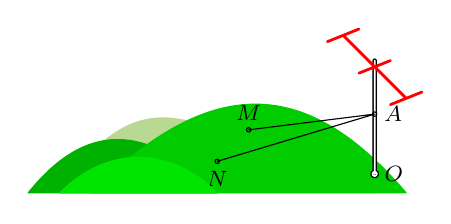
\begin{tikzpicture}[scale=.4,>=stealth, font=\footnotesize, line join=round, line cap=round]
			\filldraw[green!40!brown!50] 
			(-5,0) .. controls (-3,3) and (-1.5,2.5) .. (0,2) .. controls (1.5,2.5) and (3,2) .. (5,0) -- cycle;
			\filldraw[green!70!black] 
			(-6,0) .. controls (-4,2.5) and (-2,2) .. (0,0) -- cycle;
			\filldraw[green!80!black] 
			(-4,0) .. controls (0,4) and (3,3.5) .. (6,0) -- cycle;
			\draw[line width=.5, double](5,0.6)node[right]{$O$}circle(2pt)--(5,4.2);
			\draw[line width=1,red](4,5)--(6,3) (3.5,4.8)--(4.5,5.2) (4.5,3.8)--(5.5,4.2) (5.5,2.8)--(6.5,3.2);
			\draw(0,1)node[below]{$N$}circle(2pt)--(5,2.5)node[right]{$A$}circle(2pt)--(1,2)node[above]{$M$}circle(2pt);
			% Vẽ các ngọn đồi đậm hơn phía trước cùng
			\filldraw[green!90!black] 
			(-5,0) .. controls (-3.5,1.5) and (-1.5,1.5) .. (0,0) -- cycle;
			
	\end{tikzpicture}}
	\begin{listEX}
		\item Tính độ dài các đoạn dây cáp $MA$ và $NA$.
		\item Tính góc tạo bởi các sợi dây cáp $MA$, $NA$ với mặt phẳng sườn đồi.
	\end{listEX} 
	\loigiai{
		\begin{listEX}
			\item Ta có $\overrightarrow{MA}=(-3; 4; 3), \overrightarrow{NA}=(5; 2; 4)$, suy ra
			\begin{itemize}
				\item $MA=\sqrt{(-3)^2+4^2+3^2}=\sqrt{34} \approx 5{,}8$ m. 
				\item $NA=\sqrt{5^2+2^2+4^2}=\sqrt{45} \approx 6{,}7$ m.
			\end{itemize}
			\item  Mặt phẳng $(OMN)$ có cặp vectơ chỉ phương là $\overrightarrow{OM}=(3;-4; 3)$,  $\overrightarrow{ON}=(-5;-2; 2)$ nên có vectơ pháp tuyến $\overrightarrow{n}=[\overrightarrow{O M}, \overrightarrow{O N}]=(-2;-21;-26)$.\\        
			Gọi $\alpha$, $\beta$ lần lượt là góc tạo bởi $MA$, $NA$ với mặt phẳng $(AMN)$.\\
			Ta có
			\begin{eqnarray*}
				&\sin \alpha=\dfrac{|\overrightarrow{M A} \cdot \overrightarrow{n}|}{|\overrightarrow{M A}| \cdot|\overrightarrow{n}|} & =\dfrac{|-3 \cdot(-2)+4 \cdot(-21)+3 \cdot(-26)|}{\sqrt{(-3)^2+4^2+3^2} \cdot \sqrt{(-2)^2+(-21)^2+(-26)^2}} \\
				&&=\dfrac{156}{\sqrt{38\,114}} \Rightarrow \alpha \approx 53^{\circ}.
			\end{eqnarray*}
			Và  
			\begin{eqnarray*}
				&\sin \beta=\dfrac{|\overrightarrow{NA} \cdot \overrightarrow{n}|}{|\overrightarrow{N A}| \cdot|\overrightarrow{n}|} & =\frac{|5 \cdot(-2)+2 \cdot(-21)+4 \cdot(-26)|}{\sqrt{5^2+2^2+4^2} \cdot \sqrt{(-2)^2+(-21)^2+(-26)^2}} \\
				&&=\dfrac{156}{\sqrt{50\,445}} \Rightarrow \beta \approx 44^{\circ}. 
			\end{eqnarray*}
		\end{listEX}    
	}
\end{vd}
\dongcham{13}

% \begin{vd}
% 	Một khuôn nướng bánh mì được mô phỏng trong không gian $Oxyz$ như hình vẽ với  $S(0; 0; 0)$, $P(8; 0; 0)$, $Q(8; 18; 0)$, $T(-1;-1; 7)$, $R(9; 19; 7)$. Tính góc giữa hai cạnh kề nhau, giữa cạnh bên và mặt đáy, giữa mặt bên và mặt đáy của khuôn.
% 	\begin{center}
% 		% \includegraphics[width=6cm]{images/KhuonBanh.jpg}~
% 		\begin{tikzpicture}[>=stealth,scale=.8]
% 			\path (0,0) coordinate (S)
% 			(-20:0.5) coordinate (ex)
% 			(15:0.5) coordinate (ey)
% 			(0,0.65) coordinate (ez)
% 			($4*(ex)$) coordinate (P)
% 			($4*(ex)+9*(ey)$) coordinate (Q)
% 			($9*(ey)$) coordinate (H)
% 			($-0.5*(ex)-0.5*(ey)+3.5*(ez)$) coordinate (T)
% 			($4.5*(ex)+9.5*(ey)+3.5*(ez)$) coordinate (R)
% 			($4.5*(ex)-.5*(ey)+3.5*(ez)$) coordinate (E)
% 			($-.5*(ex)+9.5*(ey)+3.5*(ez)$) coordinate (K)
% 			;
			
% 			\foreach \x in {-3,...,12}{
% 				\draw[dashed,gray!65] ($-3*(ex)+\x*(ey)$)--($9*(ex)+\x*(ey)$);
% 				\ifnum\x>0
% 				\pgfmathsetmacro{\xt}{int(2*\x)}
% 				\draw ($\x*(ey)+(0,-1pt)$)--($\x*(ey)+(0,1pt)$) node[above,font=\tiny]{$\xt$};
% 				\ifnum \x<9
% 				\draw ($\x*(ex)+(0,-1pt)$)--($\x*(ex)+(0,1pt)$) node[below,font=\tiny]{$\xt$};
% 				\draw[dashed,gray!65] ($-3*(ey)+\x*(ex)$)--($12*(ey)+\x*(ex)$);
% 				\fi
% 				\else
% 				\pgfmathsetmacro{\xt}{int(2*\x)}
% 				\draw ($\x*(ey)+(0,-1pt)$)--($\x*(ey)+(0,1pt)$)
% 				+(-0.1,0) node[below,font=\tiny]{$\xt$};
% 				\draw ($\x*(ex)+(0,-1pt)$)--($\x*(ex)+(0,1pt)$) +(-0.1,0) node[below,font=\tiny]{$\xt$};
% 				\draw[dashed,gray!65] ($-3*(ey)+\x*(ex)$)--($12*(ey)+\x*(ex)$);
% 				\fi
% 			}
% 			\foreach \x in {-1,1,2,...,5}{
% 				\pgfmathsetmacro{\xt}{int(2*\x)}
% 				\draw ($\x*(ez)+(1pt,0)$)--($\x*(ez)+(-1pt,0)$) +(0.5pt,0) node[anchor=east,font=\tiny]{$\xt$};
% 			}
% 			\draw[->,cyan!65] ($-3*(ex)$)--($9*(ex)$);
% 			\draw[->,cyan!65] ($-3*(ey)$)--($12.5*(ey)$);
% 			\draw[->,cyan!65] ($-1.5*(ez)$)--($5.5*(ez)$);
% 			\draw[dashed](S)--(H)--(Q) (H)--(K);
% 			\draw (S)--(P)--(E)--(T)--cycle
% 			(P)--(Q)--(R)--(E)
% 			(R)--(K)--(T);
% 			\foreach \t/\g in {S/-65,P/45,Q/-60,H/-90,R/20,K/75,T/110,E/90}{
% 				\shade[ball color=blue] (\t) circle (1pt) node[shift={(\g:7pt)},font=\scriptsize]{$ \t $};
% 			}
% 		\end{tikzpicture}
% 	\end{center}
% 	\loigiai{
% 		\begin{listEX}[1]
% 			\item Tính góc giữa hai cạnh kề nhau\\
% 			$\overrightarrow{SP}=\left(8;0;0\right);\overrightarrow{SH}=\left(0;18;0\right);\overrightarrow{ST}=\left(-1;-1;7\right)$.\\
% 			$\overrightarrow{SP}\cdot\overrightarrow{SH}=0\Rightarrow \left(SP,SH\right)=90^\circ$.\\
% 			$\cos\left(SP,ST\right)=\dfrac{\left|\overrightarrow{SP}\cdot\overrightarrow{ST}\right|}{\left|\overrightarrow{SP}\right|\cdot\left|\overrightarrow{ST}\right|}=\dfrac{1}{\sqrt{51}}\Rightarrow \left(SP,ST\right)\approx 82^\circ$.\\
% 			$\cos\left(SH,ST\right)=\dfrac{\left|\overrightarrow{SH}\cdot\overrightarrow{ST}\right|}
% 			{\left|\overrightarrow{SH}\right|\cdot\left|\overrightarrow{ST}\right|}
% 			=\dfrac{1}{\sqrt{51}}\Rightarrow \left(SH,ST\right)\approx 82^\circ$.
% 			\item Tính góc giữa cạnh bên và mặt đáy\\
% 			Gọi $\alpha$ là góc giữa cạnh bên $ST$ và mặt phẳng đáy.\\
% 			$\sin\alpha=\dfrac{\left|\overrightarrow{ST}\cdot\vec{k}\right|}{\left|\overrightarrow{ST}\right|\cdot\left|\vec{k}\right|}=\dfrac{7}{\sqrt{51}}\Rightarrow \alpha\approx 78^\circ$.
% 			\item Tính góc giữa mặt bên và mặt đáy\\
% 			Gọi $\beta$ là góc giữa mặt bên và mặt phẳng đáy.\\
% 			$\vec{n}=\left[\overrightarrow{ST},\overrightarrow{SP}\right]=\left(0;56;8\right)$.\\
% 			$\cos\beta=\dfrac{\left|\overrightarrow{n}\cdot\vec{k}\right|}{\left|\overrightarrow{n}\right|\cdot\left|\vec{k}\right|}=\dfrac{\sqrt{2}}{10}\Rightarrow \beta\approx 82^\circ$.
% 		\end{listEX}
% 	}
% \end{vd}
% \dongcham{28}
\boxmini{BÀI TẬP TRẮC NGHIỆM}
\setcounter{ex}{0}
\Opensolutionfile{ans}[ans/2H5-B3-d2]

\begin{ex}
		Trong hệ trục toạ độ $Oxyz$, với mặt phẳng $(Ox y)$ là mặt đất, một máy bay cất cánh từ vị trí $A(0; 10; 0)$ với vận tốc $\vec{v}=(150; 150; 40)$. Tính góc nâng của máy bay (góc giữa hướng chuyển động bay lên của máy bay với đường băng và làm tròn kết quả đến hàng đơn vị).
		\choice
		{$10^{\circ}$}
		{$12^{\circ}$}
		{\True $11^{\circ}$}
		{$9^{\circ}$}
	\loigiai{Gọi $\alpha$ là góc nâng của máy bay.\\
		$\sin\alpha=\dfrac{\left|\overrightarrow{v}\cdot\vec{k}\right|}{\left|\overrightarrow{v}\right|\cdot\left|\vec{k}\right|}\Rightarrow \alpha\approx 10^\circ 40'$.
	}
\end{ex}


\begin{ex}
	Cho hình lập phương $ABCD.A'B'C'D'$có cạnh bằng $a$. Tính số đo góc giữa hai mặt phẳng $(BA'C)$ và $(DA'C)$.
	\choice
	{$30^\circ$}
	{$120^\circ$}
	{$90^\circ$}
	{\True $60^\circ$}
	\loigiai{
		\immini
		{ Chọn hệ tọa độ $Oxyz$ có $A\equiv O$, $ \overrightarrow{AB}$, $\overrightarrow{AD}$, $\overrightarrow{AA'}$ lần lượt cùng hướng với các vectơ đơn vị $\overrightarrow{i}$, $\overrightarrow{j}$, $\overrightarrow{k}$.\\
			Lấy $a=1$, suy ra $B(1;0;0)$, $D(0;1;0)$, $A'(0;0;1)$, $C(1;1;0)$.\\
			Mặt phẳng $(BA'C)$ có vectơ pháp tuyến là \\ $\overrightarrow{n_1}=\overrightarrow{BA'}\wedge \overrightarrow{BC}=(-1;0;-1)$.\\
			Mặt phẳng $(DA'C)$ có vectơ pháp tuyến là \\ $\overrightarrow{n_2}=\overrightarrow{DA'}\wedge \overrightarrow{DC}=(0;1;1)$.\\
			Gọi $\varphi $ là góc giữa hai mặt phẳng $(BA'C)$ và $(DA'C)$, ta có
			$ \cos\varphi =\left|{\cos\left(\overrightarrow{n_1},\overrightarrow{n_2}\right)}\right|=\dfrac{\left|{\overrightarrow{n_1} \cdot \overrightarrow{n_2}}\right|}{\left|{\overrightarrow{n_1}}\right|\cdot \left|{\overrightarrow{n_2}}\right|}=\dfrac{1}{\sqrt{2}\cdot \sqrt{2}}=\dfrac{1}{2}$.\\ Suy ra $\varphi =60^\circ$.
		}
		{ \begin{tikzpicture}[scale=1,>=stealth, font=\footnotesize, line join=round, line cap=round]
				\tkzDefPoints{0/0/A,-1.3/-1.1/B,2/-1.1/C}
				\coordinate (D) at ($(A)+(C)-(B)$);
				\coordinate (A') at ($(A)+(0,3.3)$);
				\coordinate (x) at ($(A)!1.6!(B)$);
				\coordinate (y) at ($(A)!1.2!(D)$);
				\coordinate (z) at ($(A)!1.3!(A')$);
				\tkzDrawSegments[vector style](B,x D,y A',z)
				\tkzDefPointsBy[translation=from A to A'](B,C,D){B'}{C'}{D'}
				\tkzDrawPolygon(A',B',B,C,D,D')
				\tkzDrawSegments(B',C' C',D' C,C')
				\tkzDrawSegments[dashed](A,B A,D A,A' A',C A,C B,D A',B A',D)
				\tkzDrawPoints[fill=black,size=4](A,B,D,C,A',B',C',D')
				\tkzLabelPoints[below](B,C,x)
				\tkzLabelPoints[left](B')
				\tkzLabelPoints[right](C',z)
				\tkzLabelPoints[above right](A,D,A',D',y)
			\end{tikzpicture}
		}
	}
\end{ex}

\begin{ex}
	Cho hình lập phương $MNPQ.M'N'P'Q'$ có $E$, $F$, $G$ lần lượt là trung điểm của $NN'$, $PQ$, $M'Q'$ Tính góc giữa hai đường thẳng $EG$ và $P'F$.
	\choice
	{$60^{\circ} $}
	{\True $90^{\circ} $}
	{$30^{\circ} $}
	{$45^{\circ} $}
	\loigiai{
		\immini{Chọn hệ trục tọa độ $Oxyz$ sao cho $M(0;0;0)$, $N(1;0;0)$, $Q(0;1;0)$ và $M'(0;0;1)$. Lúc đó $P(1;1;0), N'(1;0;1), Q'(0;1;1)$ và $P'(1;1;1)$.\\
			Vì $E, F, G$ lần lượt là trung điểm $NN', PQ$ và $M'Q'$ nên $E\left(1;0;\dfrac{1}{2}\right)$, $F\left(\dfrac{1}{2};1;0\right)$ và $G\left(0;\dfrac{1}{2};1\right)$.\\
			Suy ra $\vec{EG}=\left(-1;\dfrac{1}{2};\dfrac{1}{2}\right)$, $\vec{P'F}=\left(-\dfrac{1}{2};0;-1\right)$, do đó $\vec{EG}\cdot \vec{P'F}=0$ hay $(EG,P'F)=90^{\circ}$.}{\begin{tikzpicture}[line cap=round,line join=round,scale=1.5]%[Mai Hà Lan] %1.20
				%-------------- Đáy ABCD
				\tkzDefPoints{0/0/A, -0.5/-1/B, 2/0/D}
				\coordinate (C) at ($(B)+(D)-(A)$);
				%-------------- Đáy A'B'C'D'
				\tkzDefPointBy[rotation = center A angle 90](D) \tkzGetPoint{A'} %Phép quay tâm A, góc quay 90 độ, biến D thành A'
				\coordinate (B') at ($(B)+(A')-(A)$);
				\coordinate (D') at ($(D)+(A')-(A)$);
				\coordinate (C') at ($(B')+(D')-(A')$);
				%---------------
				\tkzDrawSegments[dashed](A,B A,D A,A')
				\tkzDrawPolygon(A',B',C',D')
				\tkzDrawPolygon(B,C,C',B')
				\tkzDrawSegments(D,D' C,D)
				\tkzDrawPoints(A,B,C,D,A',B',C',D')
				\tkzLabelPoint(A){$M$}
				\tkzLabelPoint(B){$N$}
				\tkzLabelPoint(C){$P$}
				\tkzLabelPoint(D){$Q$}
				\tkzLabelPoint(A'){$M'$}
				\tkzLabelPoint(B'){$N'$}
				\tkzLabelPoint(C'){$P'$}
				\tkzLabelPoint(D'){$Q'$}
				%\tkzLabelPoints(A,B,C,D,A',B',C',D')
				\tkzDefMidPoint(B,B') \tkzGetPoint{E}
				\tkzDefMidPoint(C,D) \tkzGetPoint{F}
				\tkzDefMidPoint(A',D') \tkzGetPoint{G}
				\tkzLabelPoints[above](G)
				\tkzLabelPoints[right](E,F)
				\tkzDrawSegments[dashed](E,G)
				\tkzDrawSegments(C',F)
				\tkzDrawPoints(G,E)
		\end{tikzpicture}}
	}
\end{ex}

\begin{ex}
	Cho hình hộp chữ nhật $ABCD.A'B'C'D'$ có các cạnh $AB=2,AD=3,AA'=4$. Góc giữa hai mặt phẳng $(AB'D')$ và $(A'C'D)$ là $\alpha$. Tính giá trị gần đúng của góc $\alpha$.
	\choice
	{$45,2^{\circ}$}
	{$38,1^{\circ}$}
	{\True $61,6^{\circ}$}
	{$53,4^{\circ}$}
	\loigiai{
		\immini{Gắn hình hộp chữ nhật $ABCD.A'B'C'D'$ vào hệ trục tọa độ $Oxyz$. Khi đó $A(0,0,0)$, $B(0;2;0)$, $C(3;2;0)$, $D(3;0;0)$, $A'(0;0;4)$, $B'(0;2;4)$, $C'(3;2;4)$, $D'(3;0;4)$.\\
			$\vec{AB'}=(0;2;4)$, $\vec{AD'}=(3;0;4)$, $\vec{A'C'}=(3;2;0),\vec{A'D}=(3;0;-4)$.\\
			Gọi $\overrightarrow{n}_{1}$ là vectơ pháp tuyến của $(AB'D')$. Ta có $\overrightarrow{n}_{1}=[\vec{AB'},\vec{AD'}]=(8;12;-6)$.\\
			Gọi $\overrightarrow{n}_{2}$ là vectơ pháp tuyến của $(A'C'D)$. Ta có $\overrightarrow{n}_{2}=[\vec{A'C'},\vec{A'D}]=(-8;12;-6)$.\\
			$\alpha$ là góc giữa hai mặt phẳng $(AB'D')$ và $(A'C'D)$, ta có \\
			$\cos \alpha=\left|\dfrac{\overrightarrow{n}_{1}\cdot \overrightarrow{n}_{2}}{|\overrightarrow{n}_{1}||\overrightarrow{n}_{2}|} \right|=\dfrac{29}{61}$.\\
			Vậy giá trị gần đúng của góc $\alpha$ là $61,6^{\circ}$.
		}{
	\begin{tikzpicture}
		\tkzDefPoints{0/0/A,-3/-2/D,2/-2/C,5/0/B,0/5/A',-3/3/D',2/3/C',5/5/B'}
		\tkzDrawPoints(A,B,C,D,A',B',C',D')
		\tkzLabelPoints[above right](A')
		\tkzLabelPoints[above left](B')
		\tkzLabelPoints[above](C')
		\tkzLabelPoints[above left](B,D',D)
		\tkzLabelPoints[below right](A,C)
		\tkzDrawSegments(B,C C,D D,D' C,C' B,B' A',B' B',C' C',D' D',A' B',D' A',C' C',D)
		\tkzDrawSegment[style=dashed](A,B)
		\tkzDrawSegment[style=dashed](A,D)
		\tkzDrawSegment[style=dashed](A,A')
		\tkzDrawSegment[style=dashed](A,B')
		\tkzDrawSegment[style=dashed](A,D)
		\tkzDrawSegment[style=dashed](A,D')
		\tkzDrawSegment[style=dashed](A',D)
\end{tikzpicture}}
	}
\end{ex}

\begin{ex}
		Cho hình chóp $SABCD$ có $ABCD$ là hình vuông cạnh $a$, $SA$ vuông góc $\left(ABCD\right)$, $SA=a$. Gọi $E$ và $F$ lần lượt là trung điểm $SB,SD$. Cô-sin của góc hợp bởi hai mặt phẳng $\left(AEF\right)$ và $\left(ABCD\right)$ là
		\choice
		{$\sqrt{3}$}
		{$\dfrac{\sqrt{3}}{2}$}
		{$\dfrac{1}{2}$}
		{\True $\dfrac{\sqrt{3}}{3}$}
	\loigiai{
		\immini{
			Chọn hệ trục tọa độ như hình vẽ. Ta có:
			$A\left(0;0;0\right)$, $B\left(a;0;0\right)$, $D\left(0;a;0\right)$, $S\left(0;0;a\right)$, $E\left(\dfrac{a}{2};0;\dfrac{a}{2}\right)$, $F\left(0;\dfrac{a}{2};\dfrac{a}{2}\right)$ và
			$\overrightarrow{AE}\left(\dfrac{a}{2};0;\dfrac{a}{2}\right)$, $\overrightarrow{AF}\left(0;\dfrac{a}{2};\dfrac{a}{2}\right)$.\\
			$\Rightarrow \left[\overrightarrow{AE},\overrightarrow{AF}\right]=\left(-\dfrac{a^2}{4};-\dfrac{a^2}{4};\dfrac{a^2}{4}\right)$.\\
			$\Rightarrow $ Một VTPT của mặt phẳng $\left(AEF\right)$ là $\left(1;1;-1\right)$.
			Phương trình mặt phẳng $\left(AEF\right)\colon $ $x+y-z=0$.\\
			Phương trình mặt phẳng $\left(ABCD\right)\colon z=0$.
		}{
			\begin{tikzpicture}[scale=0.8, font=\footnotesize, line join=round, line cap=round, >=stealth]
				\def \xa{-2}
				\def \xb{-1}
				\def \y{4}
				\def \z{3}
				\coordinate (A) at (0,0);
				\coordinate (B) at ($(A)+(\xa,\xb)$);
				\coordinate (Bx) at ($(B)+(\xa,\xb)$);
				\coordinate (D) at ($(A)+(\y,0)$);
				\coordinate (Dy) at ($(D)+(2,0)$);
				\coordinate (C) at ($ (B)+(D)-(A) $);
				\coordinate (S) at ($ (A)+(0,\z) $);
				\coordinate (Sz) at ($ (S)+(0,1.5) $);
				\tkzDefMidPoint(S,B)    \tkzGetPoint{E}
				\tkzDefMidPoint(S,D)    \tkzGetPoint{F}
				\draw [dashed] (B)--(A)--(D) (A)--(S) (A)--(E)--(F)--(A);
				\draw (S)--(B)--(C)--(D)--(S)--(C);
				\draw[->] (B)--(Bx) node [below right] {$x$};
				\draw[->] (D)--(Dy) node [below] {$y$};
				\draw[->] (S)--(Sz) node [right] {$z$};
				\tkzDrawPoints(S,A,B,C,D,E,F)
				\tkzLabelPoints[above right](D)
				\tkzLabelPoints[below right](C)
				\tkzLabelPoints[above left](S)
				\tkzLabelPoints[left](A)
				\tkzLabelPoints[below](B)
				\tkzLabelPoints[above right](F)
				\tkzLabelPoints[above left](E)
		\end{tikzpicture}}
		\noindent Góc hợp bởi hai mặt phẳng $\left(AEF\right)$ và $\left(ABCD\right)$ là $\alpha $, ta có $\cos \alpha =\left| \dfrac{-1}{\sqrt{3}\cdot  1}\right|=\dfrac{1}{\sqrt{3}}.$
	}
\end{ex}
\begin{ex}
	Cho hình chóp tam giác $O.ABC$ có $OA$, $OB$, $OC$ đôi một vuông góc và $OA=OB=OC$. Lấy $M$, $N$ lần lượt là trung điểm của $AB$, $OC$. Gọi $\alpha$ là góc tạo bởi $OA$ và $MN$. Tính $\cos\alpha$.
	\choice
	{\True $\dfrac{\sqrt{3}}{3}$}
	{$\dfrac{1}{3}$}
	{$\dfrac{\sqrt{3}}{4}$}
	{$\dfrac{\sqrt{3}}{2}$}
	\loigiai{
		\immini{
			Do $OA$, $OB$, $OC$ đôi một vuông góc nên chọn hệ trục toạ độ như hình vẽ. Khi đó, ta có hệ toạ độ của các điểm $O(0;0;0)$, $A(a;0;0)$, $B(0;a;0)$, $C(0;0;a)$.\\
			Suy ra $M\left(\dfrac{a}{2};\dfrac{a}{2};0\right)$, $N\left(0;0;\dfrac{a}{2}\right)$ nên $\overrightarrow{N M}=\left(\dfrac{a}{2} ; \dfrac{a}{2} ;-\dfrac{a}{2}\right)$.\\
			Suy ra $\cos \alpha=\dfrac{\dfrac{a^{2}}{2}}{\sqrt{0^{2}+0^{2}+a^{2}} \sqrt{\left(\dfrac{a}{2}\right)^{2}+\left(\dfrac{a}{2}\right)^{2}+\left(-\dfrac{a}{2}\right)^{2}}}=\dfrac{\sqrt{3}}{3}$.
		}{
			\begin{tikzpicture}[scale=0.8,>=stealth, font=\footnotesize, line join=round, line cap=round]
				%%\draw[color=gray!50,dashed] (-6,-6) grid (6,6);
				\tkzSetUpPoint[fill=black]
				\tkzDefPoints{0/0/O,3/0/C,0/3/A,-2/-2/B}
				\tkzDefMidPoint(A,B)\tkzGetPoint{M}
				\tkzDefMidPoint(O,C)\tkzGetPoint{N}
				\coordinate (x) at ($(O)!1.3!(B)$);
				\coordinate (y) at ($(O)!1.2!(C)$);
				\coordinate (z) at ($(O)!1.2!(A)$);
				\draw[line width = 0.6pt,->](B) -- (x);
				\draw[line width = 0.6pt,->](C) -- (y);
				\draw[line width = 0.6pt,->](A) -- (z);
				\tkzDrawPoints[fill=black,size=4](O,A,B,C,M,N)
				\tkzLabelPoints[above left](A)
				\tkzLabelPoints[left](B,O)
				\tkzLabelPoints[left](M)
				\tkzLabelPoints[above](N)
				\tkzLabelPoints[right](z,x)
				\tkzLabelPoints[below](y)
				\tkzLabelPoints[above right](C)
				\tkzDrawSegments[dashed](O,A O,B O,C M,N)
				\tkzDrawSegments(A,B B,C A,C)
				\tkzMarkRightAngles[size=0.16](B,O,C A,O,C B,O,A)
			\end{tikzpicture}
		}
	}
\end{ex}
\begin{ex}%[2H3K4-1]%
	Hình chóp $S.ABC$ có đáy là tam giác vuông tại $B$ có $AB=a$,  $AC =2a$. $SA$ vuông góc với mặt phẳng đáy, $SA = 2a$. Gọi $\psi$ là góc tạo bởi hai mặt phẳng $(SAC)$ và $(SBC)$. Tính $\cos\psi$.
	\choice
	{$\dfrac{1}{2}$}
	{$\dfrac{\sqrt{3}}{5}$}
	{$\dfrac{\sqrt{3}}{2}$}
	{\True $\dfrac{\sqrt{15}}{5}$}
	\loigiai{
		\immini{Chọn hệ trục tọa độ $Bxyz$ như hình vẽ.\\
			Ta tính được $B(0;0;0)$, $A(a;0;0)$, $C(0;a \sqrt{3};0)$, $S(a;0;2a)$,\\
			$\vv{SA}=(0;0;-2a)$, $\vv{SB}=(-a;0;-2a)$, $\vv{SC}=(-a;a\sqrt{3};-2a)$,\\
			$\vv{n_1}= \left[ \vv{SA} ; \vv{SC} \right] = (2a^2\sqrt{3};2a^2;0)$ là VTPT của $(SAC)$,\\
			$\vv{n_2}= \left[ \vv{SB} ; \vv{SC} \right] = (2a^2\sqrt{3};0;-a^2\sqrt{3})$ là VTPT của $(SBC)$.\\
			Ta có $$\cos \psi = \big|\cos \left[\vv{n_1};\vv{n_2}\right]\big|=\dfrac{|\vv{n_1}\vv{n_2}|}{|\vv{n_1}|\cdot |\vv{n_2}|}=\dfrac{\sqrt{15}}{5}.$$
		}{\begin{tikzpicture}[>=stealth,line join=round,line cap=round,font=\footnotesize,scale=0.8]
				\tkzDefPoints{0/0/A, 2/-2/B, 7/0/C}
				\coordinate (S) at ($(A)+(0,5)$);
				\tkzDefPointBy[homothety = center B ratio 1.7](A)
				\tkzGetPoint{E}
				\tkzDefPointBy[homothety = center B ratio 1.4](C)
				\tkzGetPoint{F}
				\coordinate (G) at ($(B)+(0,7)$);
				\tkzDrawSegments[dashed](A,C)
				\tkzDrawSegments(S,A S,B B,C S,C A,B)
				\tkzLabelPoints[below left](A,B)
				\tkzLabelPoints[below right](C)
				\tkzLabelPoints[above](S)
				\tkzMarkRightAngle(A,B,C)
				\draw[->](B)--(E);
				\draw[->](B)--(F);
				\draw[->](B)--(G);
				\draw (-1.5,1.5)node[below left]{$x$} (9,0)node[above]{$y$} (2.5,5)node[right]{$z$};
				\draw (0,2)node[above left]{$2a$};
				\draw (1.3,-1.5)node[above left]{$a$};
				\draw (3,0) node[above]{$2a$};
			\end{tikzpicture}
	}}
\end{ex}

\begin{ex}
	Cho hình chóp $S.ABCD$ có đáy $ ABCD $ là hình chữ nhật, $ AB=a $, $ BC=a\sqrt{3} $, $ SA=a $ và $ SA $ vuông góc với đáy $ ABCD $. Tính $ \sin \alpha $, với $ \alpha $ là góc tạo bởi giữa đường thẳng $ BD $ và mặt phẳng $ (SBC) $.
	\choice
	{\True $\dfrac{\sqrt{2}}{4} $}
	{$ \dfrac{\sqrt{3}}{3} $}
	{$ \dfrac{\sqrt{3}}{4} $}
	{$\dfrac{\sqrt{2}}{2} $}
	\loigiai{
		\immini{
			Đặt hệ trục tọa độ $ Oxyz $ như hình vẽ. Khi đó $A(0;0;0)$, $B(a;0;0)$, $D(0;a\sqrt{3};0)$, $S(0;0;a)$.\\
			Ta có $ \overrightarrow {BD}  = (-a;a\sqrt{3};0) = a(-1;\sqrt{3};0) $ nên đường thẳng $ BD $ có vectơ chỉ phương là $ \overrightarrow {u} = (-1;\sqrt{3};0) $.\\
			Ta có  $\overrightarrow {SB} = (a;0;-a)$, $ \overrightarrow {BC} = (0;a\sqrt{3};0) \Rightarrow \left[\overrightarrow {SB} ,\overrightarrow {BC} \right] = \left( {a^2 \sqrt{3}; 0; a^2\sqrt{3}} \right) = a^2 \sqrt{3}  (1;0;1)$. Nên mặt phẳng $ (SBC) $ có vectơ pháp tuyến là $ \overrightarrow {n} = (1;0;1) $.\\
			$ \alpha $ là góc tạo bởi giữa đường thẳng $ BD $ và mặt phẳng $ (SBC) $ thì \\
			$
			\sin \alpha = \dfrac{\left|\overrightarrow u \cdot \overrightarrow{n} \right|}{\left| {\overrightarrow{u}} \right| \cdot \left| {\overrightarrow {n}} \right|}
			= \dfrac{|( - 1)\cdot 1 + \sqrt 3 \cdot 0 + 0 \cdot1 |}{\sqrt {(- 1)^2  + (\sqrt 3)^2  + 0^2 } \cdot \sqrt {1^2  + 0^2  + 1^2}}
			= \dfrac{\sqrt 2}{4}.
			$
		}{
			\begin{tikzpicture}[scale=0.5,>=stealth]
				\tkzDefPoints{0/0/A, -3/-2/x, 7/0/y, 0/7/z}
				\coordinate (B) at ($(A)+(x)$);
				\coordinate (D) at ($(A)+(y)$);
				\coordinate (C) at ($(B)+(D)$);
				\coordinate (S) at ($(A)+(z)$);
				\coordinate (a) at ($(A)!1.4!(B)$);
				\coordinate (b) at ($(A)!1.2!(D)$);
				\coordinate (c) at ($(S)+(0,1)$);
				\tkzDrawPoints[fill=black](A,B,C,D,S)
				\draw (S)--(B)--(C)--(D)--(S) (S)--(C);
				\draw[dashed] (S)--(A)--(B)--(D)--(A);
				\draw[->] (B)--(a);
				\draw[->] (D)--(b);
				\draw[->] (S)--(c);
				\tkzLabelPoints[left](S,A,B)
				\tkzLabelPoints[below right](C)
				\tkzLabelPoints[above right](D)
				\node[above] at (a) {$y$};
				\node[below] at (b) {$x$};
				\node[left] at (c) {$z$};
			\end{tikzpicture}
		}
	}
\end{ex}

\begin{ex}
	Cho hình chóp tứ giác đều $S.ABCD$ có cạnh đáy bằng $a$, tâm $O$. Gọi $M$ và $N$ lần lượt là trung điểm $SA$ và $BC$. Biết góc giữa $MN$ và $\left(ABCD\right)$ bằng $60^{\circ}$, côsin góc giữa $MN$ và mặt phẳng $(SBD)$ bằng
	\choice
	{$\dfrac{\sqrt{41}}{41}$}
	{$\dfrac{2\sqrt{41}}{41}$}
	{$\dfrac{\sqrt{5}}{5}$}
	{\True $\dfrac{2\sqrt{5}}{5}$}
	\loigiai{
		\begin{center}
			\begin{tikzpicture}[scale=0.8, font=\footnotesize, line join=round, line cap=round, >=stealth]
				\coordinate (A) at (0,0);
				\coordinate (B) at ($(A) +(5,0)$);
				\coordinate (C) at ($(B) +(-140:2.5)$);
				\coordinate (D) at ($(A) +(-140:2.5)$);
				\coordinate (O) at ($(A)!0.5!(C)$);
				\coordinate (S) at ($(O)+(0,4)$);
				\coordinate (M) at ($(S)!0.5!(A)$);
				\coordinate (N) at ($(B)!0.5!(C)$);
				\coordinate (I) at ($(A)!0.5!(O)$);
				\coordinate (K) at ($(S)!0.5!(O)$);
				\coordinate (x) at ($(A)!1.4!(C)$);
				\coordinate (y) at ($(D)!1.4!(B)$);
				\coordinate (z) at ($(O)!1.4!(S)$);
				\foreach \x in {A,B,C,D,O,M,N}{
					\draw[fill] (\x) circle(1pt);
				}
				\draw (D)--(C)--(B) (S)--(B) (S)--(C) (S)--(D);
				\draw[dashed] (A)--(B) (A)--(D) (S)--(A) (S)--(O) (M)--(N) (B)--(D) (A)--(C);
				\draw[->]  (C)--(x) node[right]{$x$};
				\draw[->]  (B)--(y) node[above]{$y$};
				\draw[->]  (S)--(z) node[right]{$z$};
				\path
				node at (A) [left]{$A$}
				node at (B) [below]{$B$}
				node at (C) [below]{$C$}
				node at (D) [below left]{$D$}
				node at (S) [left]{$S$}
				node at (O) [below]{$O$}
				node at (M) [below left]{$M$}
				node at (N) [below right]{$N$};
			\end{tikzpicture}
		\end{center}
		Chọn hệ trục tọa độ như hình vẽ, đặt $OS=k$ $(k>0)$.\\
		Ta có $A\left(-\dfrac{a\sqrt{2}}{2};0;0\right)$, $B\left(0;\dfrac{a\sqrt{2}}{2};0\right)$, $C\left(\dfrac{a\sqrt{2}}{2};0;0\right)$, $D\left(0;-\dfrac{a\sqrt{2}}{2};0\right)$, $S\left(0;0;k\right)$,\\ $M\left(-\dfrac{a\sqrt{2}}{4};0;\dfrac{k}{2}\right)$ và $N\left(\dfrac{a\sqrt{2}}{4};\dfrac{a\sqrt{2}}{4};0\right)$.\\
		Ta có $\vec{u}_{MN}= \vec{MN}=\left(\dfrac{a\sqrt{2}}{2}; \dfrac{a\sqrt{2}}{4};-\dfrac{k}{2}\right)$ và $\vec{n}_{ABCD} = (0;0;1)$.\\
		Ta có \begin{eqnarray*}
			\sin \left(MN;(ABCD)\right)= \dfrac{\left|\vec{u}_{MN} \cdot \vec{n}_{ABCD}\right|}{\left|\vec{u}_{MN}\right| \cdot \left|\vec{n}_{ABCD}\right|} & \Leftrightarrow & \sin 60^{\circ} =\dfrac{\dfrac{k}{2}}{\sqrt{\dfrac{9a^2}{16}+\dfrac{k^2}{4}}} \\
			&\Leftrightarrow & k =  \dfrac{a\sqrt{30}}{2}.
		\end{eqnarray*}
		Ta có $\vec{n}_{SBD}=(1;0;0)$, do đó
		\begin{eqnarray*}
			\sin \left(MN,(SBD)\right)= \dfrac{\left|\vec{u}_{MN} \cdot \vec{n}_{SBD}\right|}{\left|\vec{u}_{MN}\right| \cdot \left|\vec{n}_{SBD}\right|} & \Leftrightarrow & \sin \left(MN,(SBD)\right)= \dfrac{\dfrac{a\sqrt{2}}{2}}{\sqrt{\dfrac{5a^2}{2}}} = \dfrac{\sqrt{5}}{5}.
		\end{eqnarray*}
		$\Rightarrow  \cos \left(MN,(SBD)\right) = \dfrac{2\sqrt{5}}{5}$. (do góc nhọn nên $cos$ dương)
	}
\end{ex}
\begin{ex}
	Cho hình chóp $S.ABCD$ có đáy là hình thang vuông tại $A$ và $B$, $AB=BC=a$, $AD=2a, \ \ SA$ vuông góc với mặt đáy $(ABCD)$, $SA=a$. Gọi $M,N$ lần lượt là trung điểm của $SB$ và $CD$. Tính cosin của góc giữa $MN$ và $(SAC)$.
	\choice
	{$\dfrac{2}{\sqrt{5}}$}
	{$\dfrac{1}{\sqrt{5}}$}
	{$\dfrac{3 \sqrt{5}}{10}$}
	{\True $\dfrac{\sqrt{55}}{10}$}
	\loigiai{
		\immini{
			Chọn hệ trục $Oxyz$ như hình vẽ, với $O \equiv A$. \\
			Khi đó ta có: $A(0;0;0)$, $B(a;0;0)$, $C(a;a;0)$, $D(0;2a;0)$, $S(0;0;a)$. \\
			Khi đó: $M \left(\dfrac{a}{2};0; \dfrac{a}{2} \right)$, $N \left(\dfrac{a}{2}; \dfrac{3a}{2};0 \right)$. \\
			Ta có: $- \dfrac{1}{a} \vec{SA}=(0;0;1)= \vec{u}$; $\dfrac{1}{a} \vec{SC}=(1;1;-1)= \vec{v}$. \\
			Gọi $\vec{n}$ là vectơ pháp tuyến của mặt phẳng $(SAC)$ ta có $\vec{n}= \left[\vec{u}, \vec{v} \right]=(-1;-1;0)$. \\
			Lại có: $\dfrac{2}{a} \vec{MN}=(0;3;-1)= \vec{w}$. \\
			Gọi $\alpha $ là góc giữa $MN$ và $(SAC)$ ta có: $\sin \alpha = \dfrac{\left| \vec{n}. \vec{w} \right|}{\left| \vec{n} \right|. \left| \vec{w} \right|}= \dfrac{3}{2 \sqrt{5}} \Rightarrow \cos \alpha = \dfrac{\sqrt{55}}{10}.$
		}
		{
			\begin{tikzpicture}[scale=0.7,>=stealth]
				\tkzDefPoints{0/0/A, 5/0/D, -2/-2/B, 1/-2/C}
				\tkzDefShiftPoint[A](90:4){S}
				\draw [thick] [->] (0,4)--(0,5) node[right] {$z$};
				\draw [thick] [->] (5,0)--(6,0) node[above] {$y$};
				\draw [thick] [->] (-2,-2)--(-3,-3) node[above] {$x$};
				\tkzDefMidPoint(S,B)\tkzGetPoint{M}
				\tkzDefMidPoint(C,D)\tkzGetPoint{N}
				\tkzDrawSegments(S,B S,C S,D B,C C,D)
				\tkzDrawSegments[dashed](B,A A,D S,A M,N)
				\tkzDrawPoints(A,B,C,D,S,M,N)
				\tkzLabelPoints[below](A, B, C)
				\tkzLabelPoints[above right](D,N)
				\tkzLabelPoints[left](S,M)
				\tkzLabelSegments[right](A,B S,A){$a$}
				\tkzLabelSegment[below](C,B){$a$}
				\tkzLabelSegment[above](A,D){$2a$}
			\end{tikzpicture}
		}
	}
\end{ex}
\Closesolutionfile{ans}